\section{Introducci\'on}
\subsection{Grafos}

\begin{frame}
\frametitle{Grafos}

Un grafo $G$ se define como un par $V,E$ donde $V$ es un conjunto de nodos, unidos por los ejes del conjunto $E$.

\vspace{11pt}

\begin{figure}[h]
	\centering	
	\samplegraph
\end{figure}

\end{frame} 

\begin{frame}
\frametitle{Coloreo}

El problema de coloreo consiste en asignar un \textbf{color} a cada nodo de manera tal que dos nodos adyacentes tengan colores distintos. Se busca minimizar la cantidad de colores a utilizar.

\begin{figure}[h]
	\centering	
	\samplecoloredgraph
\end{figure}

\end{frame}	

\begin{frame}
\frametitle{Coloreo}

Pintando el mapa de sudam�rica...

\begin{figure}[h]
	\centering
	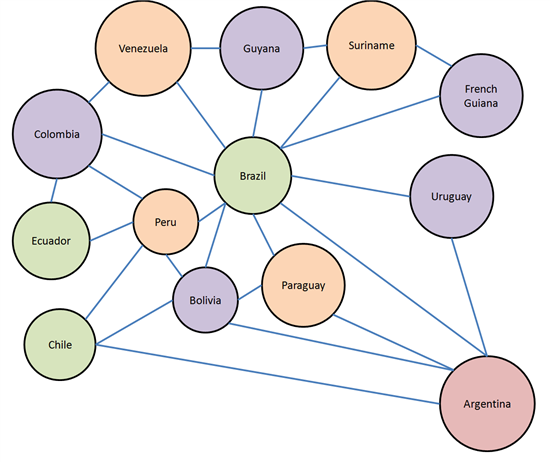
\includegraphics[scale=0.5]{../imgs/southamerica.png}
\end{figure}


\end{frame}


\begin{frame}
\frametitle{Grafos particionados}

Un grafo \textbf{particionado} es un grafo en el que el conjunto de nodos se encuentra dividido en particiones $P_0, \ldots,P_q$.

\vspace{21pt}

\begin{figure}[h]
	\centering	
	\samplepartitionedgraph
\end{figure}

\end{frame}

\begin{frame}
\frametitle{Coloreo particionado}

El problema de coloreo \textbf{particionado} consiste en, dado un grafo particionado, asignar un \textbf{color} a un solo nodo por particion, de manera tal que dos nodos adyacentes no usen colores iguales. Se busca minimizar la cantidad de colores a utilizar.

\begin{figure}[h]
	\centering	
	\samplepartitionedcoloredgraph
\end{figure}

\end{frame}

\subsection{Motivaci�n}

\begin{frame} 
\frametitle{Redes WDM}

Wavelength-division multiplexing (WDM) permite multiplexar distintas se�ales �pticas sobre un mismo enlace f�sico utilizando distintas frecuencias para cada uno.

\begin{figure}[h]
	\centering
	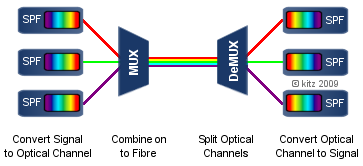
\includegraphics[scale=0.5]{../imgs/wdm.png}
\end{figure}

Se tiene una red compuesta por nodos en la que las conexiones entre ellos utilizan esta tecnolog�a. 

\end{frame} 

\begin{frame} 
\frametitle{Problema}

Se tiene un conjunto de pedidos de conexiones entre nodos, donde cada conexi�n debe usar una �nica frecuencia a lo largo de todo el camino, y si dos conexiones comparten algun enlace f�sico deben usar frecuencias distintas.

El objetivo es determinar un conjunto de rutas tal que se minimice la cantidad de frecuencias distintas usadas.

\begin{figure}[h]
	\centering
	\samplenetwork
\end{figure}

\end{frame} 

\begin{frame} 
\frametitle{Resoluci�n en dos partes}

Li y Sinha propusieron una soluci�n en dos partes para este problema:
\begin{enumerate}
\item{Generar un conjunto de rutas posibles entre cada par de nodos a conectar}
\item{Elegir una ruta de cada conjunto de manera tal que se minimice la cantidad de frecuencias necesarias}
\end{enumerate}

\end{frame} 

\begin{frame} 
\frametitle{Generaci�n de rutas}

Mediante una heur�stica, se genera una cierta cantidad de caminos distintos entre cada par de nodos que se desean conectar. Pueden usarse criterios de camino m�nimo o de maximum edge disjoint path.

\begin{figure}[h]
	\centering
	\samplenetworkroutes
\end{figure}

\end{frame} 

\begin{frame} 
\frametitle{Asignaci�n de frecuencias}

El siguiente paso es elegir una ruta entre cada par de nodos y asignarle una frecuencia, de manera tal que dos rutas distintas con la misma frecuencia no compartan ning�n enlace.

Esto puede modelarse como un problema de coloreo particionado:
\begin{itemize}
\item{Los nodos representan las rutas}
\item{Las rutas est�n agrupadas en particiones seg�n qu� conexi�n satisfacen}
\item{Los ejes indican que las rutas comparten al menos un enlace y no pueden compartir frecuencia}
\item{Las frecuencias se modelan mediante los colores}
\end{itemize}

\end{frame} 

\begin{frame} 
\frametitle{Asignaci�n de frecuencias}

Nuestro ejemplo puede resolverse usando una �nica frecuencia...

\begin{figure}[h]
		\centering	
		\alt<1>{\networkpcpgraph}{\networkpcpcoloredgraph}
\end{figure}

\begin{figure}[h]
	\centering
	\alt<1>{\samplenetworkroutes}{\solvednetwork}
\end{figure}

\uncover<2>{}

\end{frame}